% ---
% Reemplaza líneas 3458–3462 de Docs/Technical_Report.tex.
% Decisiones y hallazgos que lo respaldan: D-036, D-037, H-042, H-043, H-053, H-054.
% ---

\subsection{Clasificación}
\label{sec:rendimiento_clasificacion}

% fuente: H-042; 7_test.csv, 7_cv_resumen.csv
El protocolo de clasificación evalúa las cinco representaciones bajo una misma arquitectura de perceptrón multicapa ($k \to 32 \to 16 \to 1$) optimizada con entropía cruzada binaria ponderada. Los resultados sobre el conjunto de prueba oficial se detallan en el cuadro~\ref{tab:m7_clasificacion} y las diferencias pareadas correspondientes en el cuadro~\ref{tab:m7_diferencias}. En el subconjunto de masas, la condición de referencia C1 alcanza un AUC-ROC en el conjunto de prueba de 0.651 [IC 95\,\%: 0.578, 0.724] (0.652 $\pm$ 0.068 en validación cruzada), mientras que C2 obtiene 0.641 [0.572, 0.710] y C3 registra 0.646 [0.572, 0.721]. Las representaciones cuánticas obtienen un desempeño inferior: C4 alcanza un AUC de 0.530 [0.473, 0.587] (0.565 $\pm$ 0.079 en validación cruzada) y C5 logra 0.581 [0.521, 0.644] (0.563 $\pm$ 0.024 en validación cruzada). En masas, el clasificador sobre C4 no se distingue del azar en el conjunto de prueba.

% fuente: H-042; 7_test.csv, 7_cv_resumen.csv
En el subconjunto de calcificaciones, el desempeño general es más elevado en todas las condiciones. La condición C1 alcanza un AUC en el conjunto de prueba de 0.769 [0.694, 0.836] (0.742 $\pm$ 0.038 en validación cruzada), C2 obtiene 0.788 [0.719, 0.851] (0.758 $\pm$ 0.046 en validación cruzada) y C3 registra 0.758 [0.685, 0.826] (0.739 $\pm$ 0.036 en validación cruzada). Por su parte, las representaciones cuánticas descienden a 0.633 [0.558, 0.700] en C4 (0.640 $\pm$ 0.041 en validación cruzada) y a 0.652 [0.571, 0.725] en C5 (0.667 $\pm$ 0.035 en validación cruzada).

% fuente: H-042; 7_test_diferencias.csv
El comportamiento del control nulo resulta consistente con lo esperado: las diferencias pareadas entre C2 y C1 en el conjunto de prueba, de $-0.011$ [$-0.061$, $0.038$] ($p = 0.659$) en masas y de $0.020$ [$-0.026$, $0.067$] ($p = 0.377$) en calcificaciones, no resultan estadísticamente distinguibles de cero, como cabe esperar de una rotación, que no cambia la información disponible para el clasificador. En contraste, las representaciones cuánticas presentan pérdidas significativas respecto a C1: en masas, C4 $-$ C1 es de $-0.122$ [$-0.202$, $-0.044$] ($p = 0.003$) y C5 $-$ C1 es de $-0.070$ [$-0.140$, $-0.004$] ($p = 0.044$); en calcificaciones, C4 $-$ C1 es de $-0.135$ [$-0.208$, $-0.061$] ($p = 0.001$) y C5 $-$ C1 es de $-0.118$ [$-0.182$, $-0.046$] ($p < 0.001$). Frente a C3 las diferencias son comparables: en masas, $-0.116$ para C4 ($p = 0.006$) y $-0.065$ para C5 ($p = 0.058$); en calcificaciones, $-0.124$ para C4 ($p = 0.001$) y $-0.108$ para C5 ($p = 0.004$). La diferencia entre ambas condiciones cuánticas (C5 $-$ C4) no resulta estadísticamente significativa en ninguno de los subconjuntos: $0.051$ [$-0.027$, $0.128$] en masas y $0.017$ [$-0.061$, $0.098$] ($p = 0.679$) en calcificaciones.

% fuente: H-042; 7_test_diferencias.csv
Al considerar el problema de comparaciones múltiples sobre la familia de las cuatro diferencias cuánticas frente a C1 (C4 masas con $p \approx 0.003$, C4 calcificaciones con $p \approx 0.001$, C5 calcificaciones con $p < 0.001$ y C5 masas con $p \approx 0.044$), el procedimiento escalonado de Holm mantiene la significancia estadística de las cuatro diferencias a un nivel global $\alpha = 0.05$. Bajo la corrección más estricta de Bonferroni ($0.044 \times 4 \approx 0.18$), la diferencia de C5 en masas se sitúa en el límite y deja de ser estadísticamente significativa (figuras~\ref{fig:m7_auc} y~\ref{fig:m7_roc_test}).

% Generado por Code/tools/tablas_latex.py desde 7_test.csv y 7_cv_resumen.csv. No editar a mano: volver a correr el script.
\begin{table}[H]
\centering
\small
\caption{Clasificación con el mismo MLP sobre las cinco representaciones (M7, $k = 12$, D-036).}
\label{tab:m7_clasificacion}
\begin{adjustbox}{max width=\linewidth}
\begin{tabular}{l c c r r r r}
\toprule
Condición & AUC en VC & AUC en prueba [IC 95\,\%] & F1 & Exactitud & Precisión & Sensibilidad \\
\midrule
\multicolumn{7}{l}{\textit{Masas}} \\
\quad C1 & 0.652 $\pm$ 0.068 & 0.651 [0.578, 0.724] & 0.519 & 0.638 & 0.536 & 0.503 \\
\quad C2 & 0.641 $\pm$ 0.059 & 0.641 [0.572, 0.710] & 0.512 & 0.616 & 0.507 & 0.517 \\
\quad C3 & 0.648 $\pm$ 0.055 & 0.646 [0.572, 0.721] & 0.502 & 0.606 & 0.493 & 0.510 \\
\quad C4 & 0.565 $\pm$ 0.079 & 0.530 [0.473, 0.587] & 0.386 & 0.529 & 0.392 & 0.381 \\
\quad C5 & 0.563 $\pm$ 0.024 & 0.581 [0.521, 0.644] & 0.456 & 0.571 & 0.450 & 0.463 \\
\multicolumn{7}{l}{\textit{Calcificaciones}} \\
\quad C1 & 0.742 $\pm$ 0.038 & 0.769 [0.694, 0.836] & 0.665 & 0.666 & 0.551 & 0.837 \\
\quad C2 & 0.758 $\pm$ 0.046 & 0.788 [0.719, 0.851] & 0.669 & 0.693 & 0.584 & 0.783 \\
\quad C3 & 0.739 $\pm$ 0.036 & 0.758 [0.685, 0.826] & 0.652 & 0.653 & 0.541 & 0.822 \\
\quad C4 & 0.640 $\pm$ 0.041 & 0.633 [0.558, 0.700] & 0.504 & 0.607 & 0.504 & 0.504 \\
\quad C5 & 0.667 $\pm$ 0.035 & 0.652 [0.571, 0.725] & 0.565 & 0.571 & 0.472 & 0.705 \\
\bottomrule
\end{tabular}
\end{adjustbox}
\par\smallskip
\parbox{0.95\linewidth}{\footnotesize VC: media $\pm$ desviación estándar sobre los 5 folds de M4. Prueba: el conjunto oficial, usado una sola vez por modelo; el intervalo es un \textit{bootstrap} por paciente con 2{,}000 réplicas. Umbral de 0.5 para F1, exactitud, precisión y sensibilidad.}
\end{table}


% Generado por Code/tools/tablas_latex.py desde 7_test_diferencias.csv. No editar a mano: volver a correr el script.
\begin{table}[H]
\centering
\small
\caption{Diferencias pareadas de AUC en el conjunto de prueba (M7).}
\label{tab:m7_diferencias}
\begin{adjustbox}{max width=\linewidth}
\begin{tabular}{l r c r}
\toprule
Comparación & Diferencia & IC 95\,\% & $p$ bilateral \\
\midrule
\multicolumn{4}{l}{\textit{Masas}} \\
\quad C4 $-$ C1 & $-$0.122 & [$-$0.202, $-$0.044] & 0.003 \\
\quad C4 $-$ C3 & $-$0.116 & [$-$0.193, $-$0.041] & 0.006 \\
\quad C5 $-$ C1 & $-$0.070 & [$-$0.140, $-$0.004] & 0.044 \\
\quad C5 $-$ C3 & $-$0.065 & [$-$0.139, 0.002] & 0.058 \\
\quad C2 $-$ C1 & $-$0.011 & [$-$0.061, 0.038] & 0.659 \\
\quad C3 $-$ C1 & $-$0.005 & [$-$0.044, 0.032] & 0.796 \\
\quad C5 $-$ C4 & 0.051 & [$-$0.027, 0.128] & 0.180 \\
\multicolumn{4}{l}{\textit{Calcificaciones}} \\
\quad C4 $-$ C1 & $-$0.135 & [$-$0.208, $-$0.061] & 0.001 \\
\quad C4 $-$ C3 & $-$0.124 & [$-$0.195, $-$0.051] & 0.001 \\
\quad C5 $-$ C1 & $-$0.118 & [$-$0.182, $-$0.046] & $<$0.001 \\
\quad C5 $-$ C3 & $-$0.108 & [$-$0.177, $-$0.035] & 0.004 \\
\quad C2 $-$ C1 & 0.020 & [$-$0.026, 0.067] & 0.377 \\
\quad C3 $-$ C1 & $-$0.010 & [$-$0.034, 0.014] & 0.377 \\
\quad C5 $-$ C4 & 0.017 & [$-$0.061, 0.098] & 0.679 \\
\bottomrule
\end{tabular}
\end{adjustbox}
\par\smallskip
\parbox{0.95\linewidth}{\footnotesize Las diferencias usan las mismas réplicas del \textit{bootstrap} por paciente para ambas condiciones. $p \approx 2\min(q, 1 - q)$, con $q$ la fracción de réplicas con diferencia positiva; no está corregido por comparaciones múltiples.}
\end{table}


\begin{figure}[htbp]
\centering
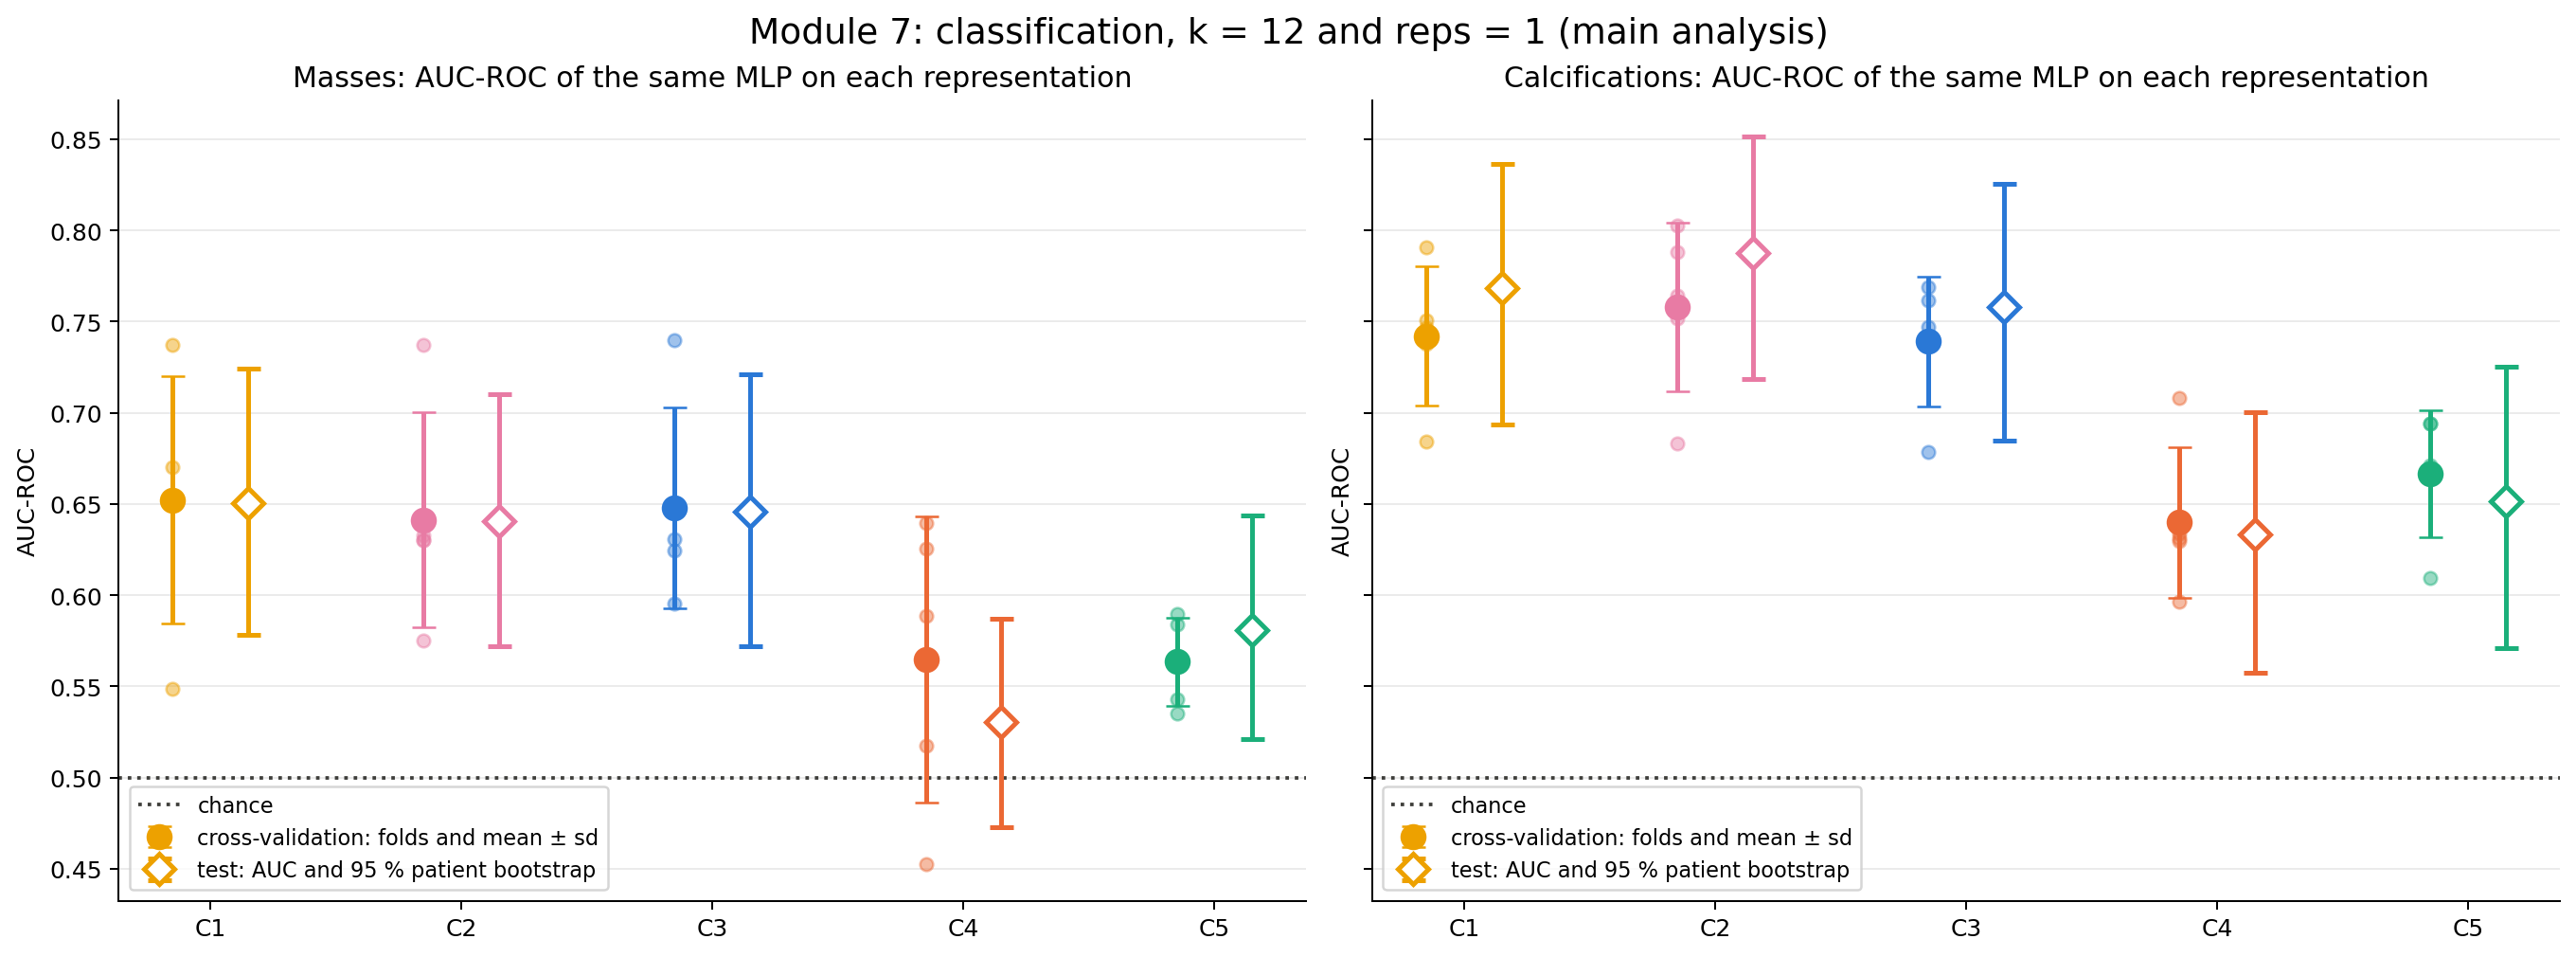
\includegraphics[width=\textwidth]{Figures/M7_auc.png}
\caption{Comparación de AUC-ROC entre las cinco condiciones evaluadas en validación cruzada y en el conjunto de prueba para masas y calcificaciones.}
\label{fig:m7_auc}
\end{figure}

\begin{figure}[htbp]
\centering
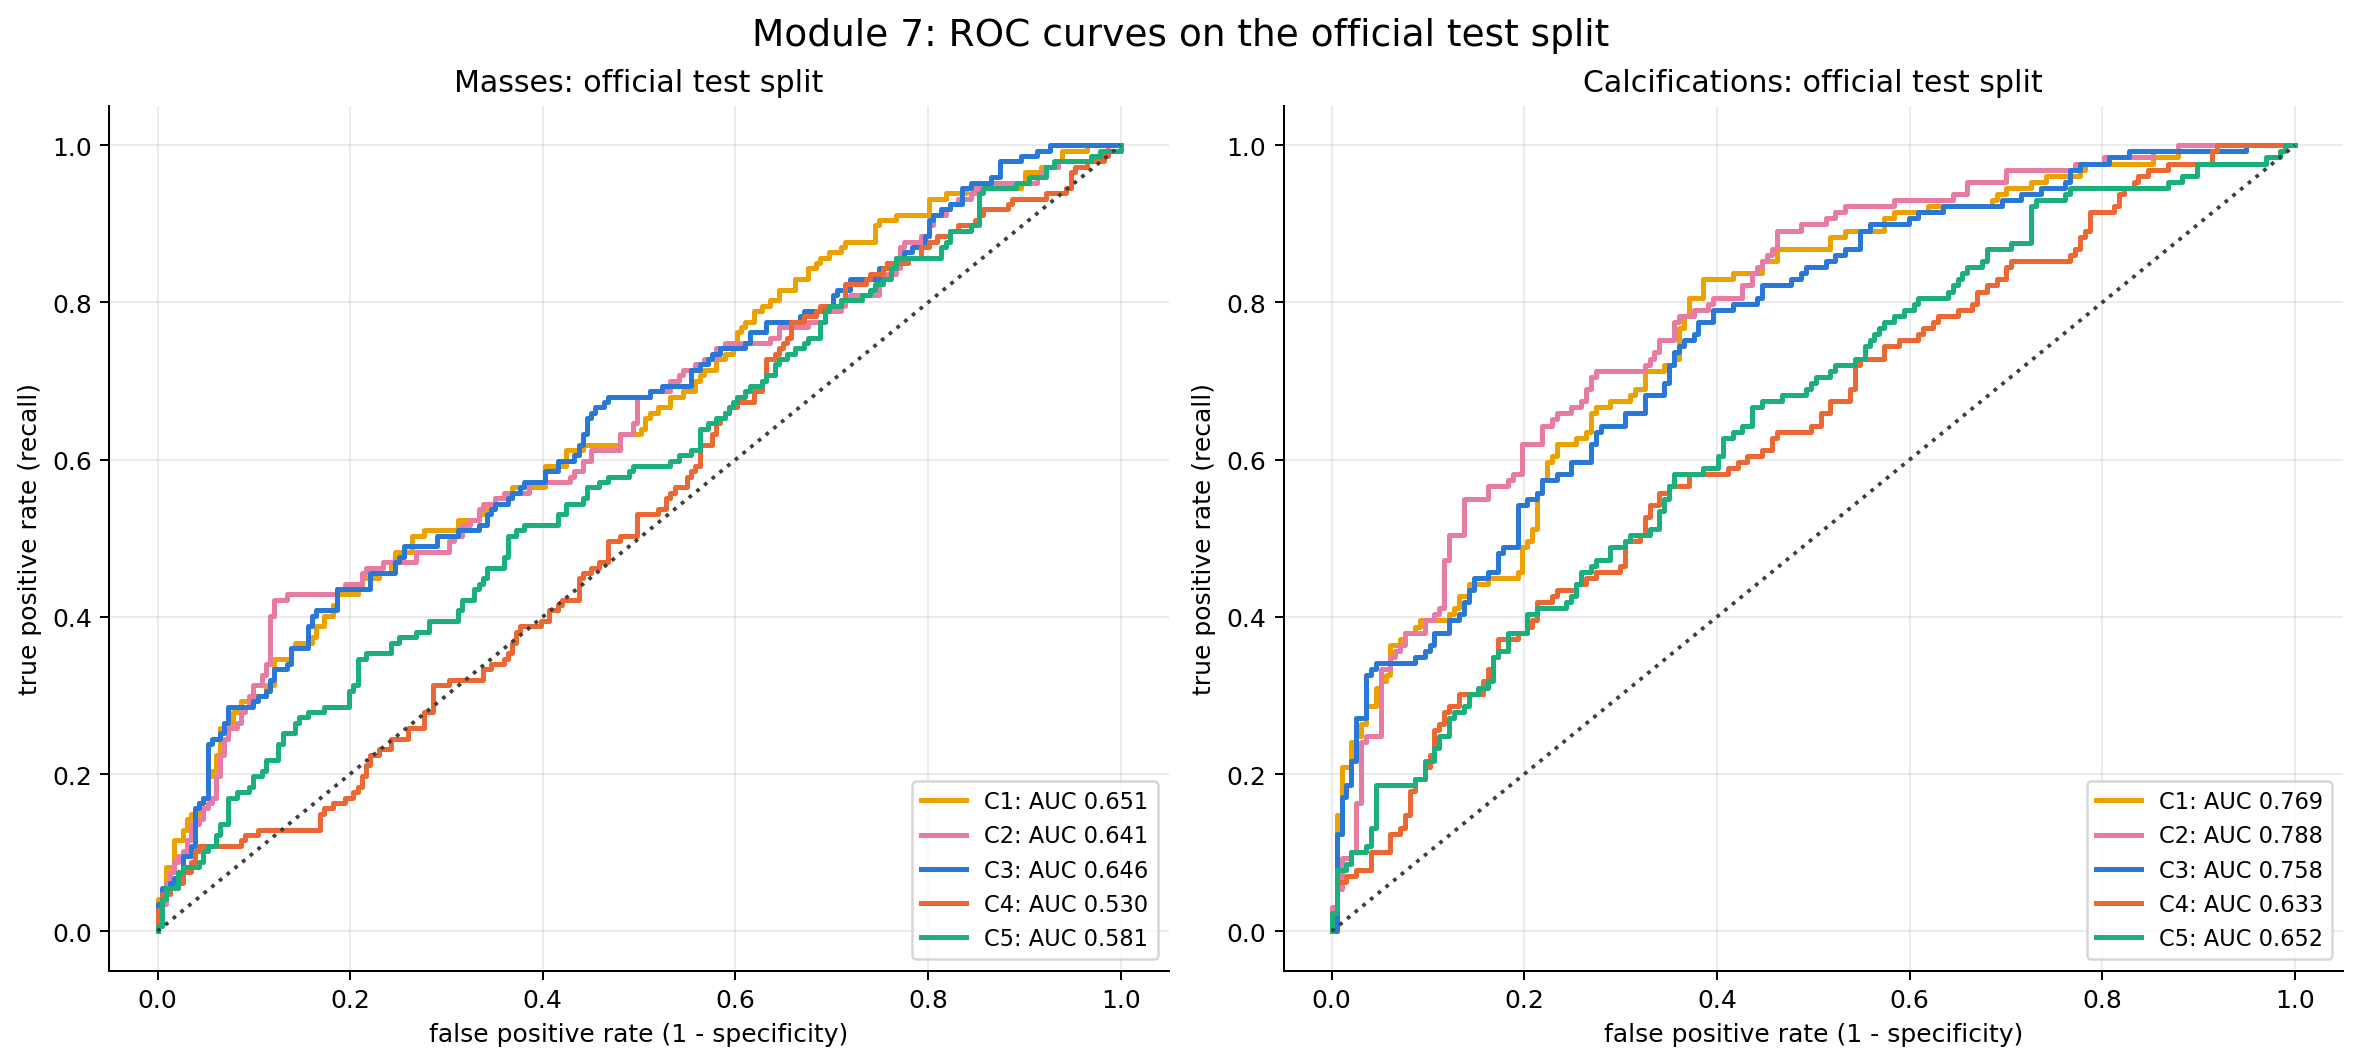
\includegraphics[width=\textwidth]{Figures/M7_roc_test.png}
\caption{Curvas ROC sobre el conjunto de prueba oficial para masas y calcificaciones bajo las cinco condiciones de representación.}
\label{fig:m7_roc_test}
\end{figure}

% fuente: H-043; 7_cv_resumen.csv, 7_test.csv, 7_test_diferencias.csv
El análisis de sensibilidad indica que la brecha observada entre condiciones clásicas y cuánticas se mantiene estable ante las variaciones evaluadas en la inicialización estocástica, la arquitectura de capas, la estandarización de las entradas y el régimen de épocas de entrenamiento. La dispersión del AUC medio en validación cruzada atribuible a la semilla del clasificador (semillas 42 a 46) no excede 0.039 en ninguna condición, lo que representa menos de la mitad de la brecha observada entre las condiciones clásicas y cuánticas (0.08 a 0.10). El empleo de arquitecturas alternativas de perceptrón multicapa (16-8 y 64-32) y el entrenamiento sin estandarización previa de entradas preservan exactamente el orden relativo de las condiciones. Por otra parte, forzar el entrenamiento a 200 épocas sin parada temprana no favorece a los modelos cuánticos: C4 y C5 deterioran su AUC medio a 0.533 y 0.557 en masas, y a 0.596 y 0.631 en calcificaciones, mientras que C1 se mantiene o mejora (0.680 en masas). Los modelos sobre representaciones cuánticas detienen su entrenamiento temprano debido a que la pérdida en el conjunto de validación cesa de mejorar, y no por subentrenamiento.

% fuente: H-043; 7_test.csv, 7_test_diferencias.csv
Al profundizar el \textit{ansatz} a dos repeticiones (\texttt{reps} = 2), la dispersión en datos reales con el vector de parámetros $\boldsymbol\theta$ fijado disminuye en C4 (de 0.058 a 0.047 en masas) y se incrementa en C5 (de 0.180 a 0.196). En clasificación, C5 mejora en el conjunto de prueba (de 0.581 a 0.603 en masas y de 0.652 a 0.682 en calcificaciones), si bien sus intervalos de diferencia frente a C1 se mantienen negativos: $-0.048$ [$-0.093$, $-0.005$] en masas y $-0.086$ [$-0.141$, $-0.034$] en calcificaciones. La condición C4 no presenta cambios apreciables. Finalmente, al reducir la dimensionalidad a $k = 8$ qubits, las condiciones clásicas prácticamente no varían, mientras que C4 tiende a empeorar en calcificaciones, alcanzando 0.561 en el conjunto de prueba con una diferencia de $-0.070$ [$-0.141$, $+0.0005$] respecto a $k = 12$, cuyo intervalo llega al cero. En este régimen de $k = 8$, las condiciones cuánticas se ubican entre 0.07 y 0.19 por debajo de C1 en el conjunto de prueba, lo cual es consistente con la observación de que una mayor dispersión geométrica en el espacio de expectativas no garantiza una mejora en la capacidad de discriminación del clasificador supervisado (figura~\ref{fig:m7_sensitivity}).

\begin{figure}[htbp]
\centering
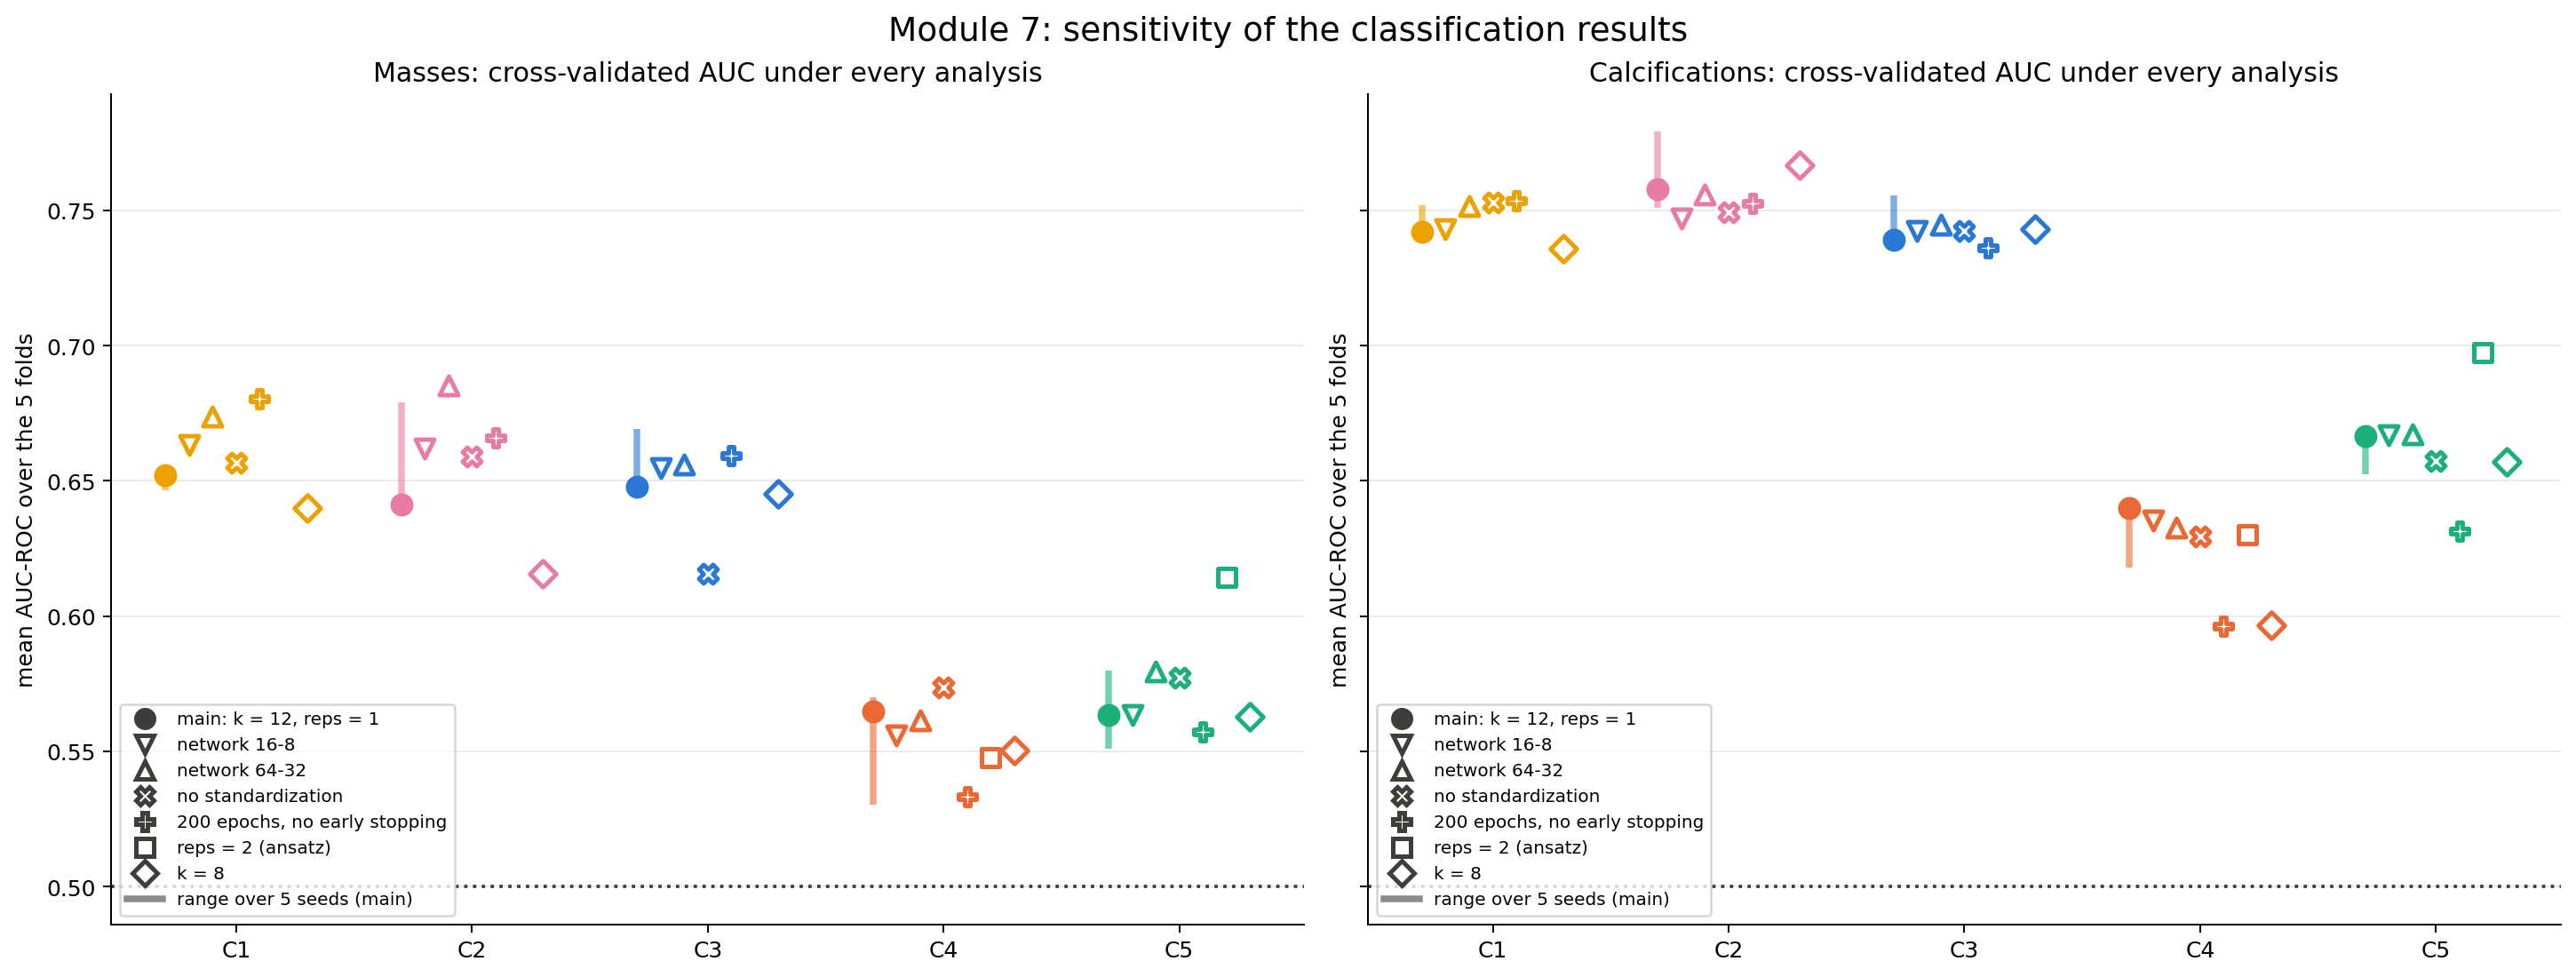
\includegraphics[width=\textwidth]{Figures/M7_sensitivity.png}
\caption{Análisis de sensibilidad del rendimiento de clasificación frente a cambios de semilla, arquitectura de red, escalado, épocas fijas, profundidad de circuito (\texttt{reps} = 2) y dimensión de entrada ($k = 8$).}
\label{fig:m7_sensitivity}
\end{figure}

% fuente: H-053; X7_resumen.csv, X7_sorteos.csv
% Generado por Code/tools/tablas_latex.py desde X7_resumen.csv. No editar a mano: volver a correr el script.
\begin{table}[H]
\centering
\small
\caption{Dependencia del AUC de C4 y C5 respecto al sorteo de $\theta$: 10 sorteos, mismo MLP y mismos folds que el M7.}
\label{tab:x7_theta}
\begin{adjustbox}{max width=\linewidth}
\begin{tabular}{l l c c r r r}
\toprule
Subconjunto & Mapa & Semilla 42 (lugar) & Mín.--máx. & Rango ($\theta$) & Rango (MLP) & C1 $-$ mejor \\
\midrule
Masas & C4 & 0.565 (6.\textsuperscript{o}) & 0.546--0.589 & 0.042 & 0.039 & 0.064 \\
Masas & C5 & 0.563 (9.\textsuperscript{o}) & 0.557--0.624 & 0.068 & 0.029 & 0.028 \\
Calcificaciones & C4 & 0.640 (6.\textsuperscript{o}) & 0.566--0.676 & 0.110 & 0.022 & 0.066 \\
Calcificaciones & C5 & 0.667 (1.\textsuperscript{o}) & 0.627--0.667 & 0.040 & 0.018 & 0.075 \\
\bottomrule
\end{tabular}
\end{adjustbox}
\par\smallskip
\parbox{0.95\linewidth}{\footnotesize AUC medio en validación cruzada; el conjunto de prueba no se usó. Rango (MLP): variación entre las 5 semillas del MLP con el $\theta$ del diseño.}
\end{table}


% fuente: H-053; X7_resumen.csv, X7_sorteos.csv
La evaluación de diez sorteos aleatorios independientes del vector de parámetros $\boldsymbol\theta$ (semillas 42 a 51) sobre los mismos pliegues de validación cruzada revela que $\boldsymbol\theta$ constituye una fuente de variación relevante, como se expone en el cuadro~\ref{tab:x7_theta}. El rango de variación del AUC debido a la elección de $\boldsymbol\theta$ oscila entre 0.040 y 0.110 (0.042 en C4 masas, 0.068 en C5 masas, 0.110 en C4 calcificaciones y 0.040 en C5 calcificaciones), igualando o superando la variación inducida por la semilla del clasificador (0.018 a 0.039). La semilla 42 establecida en el diseño inicial no constituye un caso sesgado: ocupa la sexta posición en C4 para ambos subconjuntos, la novena en C5 masas y la primera en C5 calcificaciones. Fundamentalmente, ninguno de los 40 sorteos evaluados alcanza el AUC de C1 (0.652 en masas y 0.742 en calcificaciones) ni de C3: el mejor sorteo queda entre 0.028 y 0.075 por debajo de C1, y el déficit frente a C1 se sitúa entre 0.03 y 0.18 según el sorteo. Asimismo, la correlación de Spearman entre la dispersión de $\langle Z_i \rangle$ y el AUC entre sorteos resulta no significativa en todos los casos ($p > 0.29$: 0.09 y $-0.02$ en masas; 0.03 y $-0.37$ en calcificaciones). Cabe destacar que los productos internos y las matrices de kernel no dependen de $\boldsymbol\theta$, dado que el operador unitario $V(\boldsymbol\theta)$ se cancela en el cálculo de fidelidades ($V(\boldsymbol\theta)^\dagger V(\boldsymbol\theta) = I$) (figura~\ref{fig:x7_theta_draws}).

\begin{figure}[htbp]
\centering
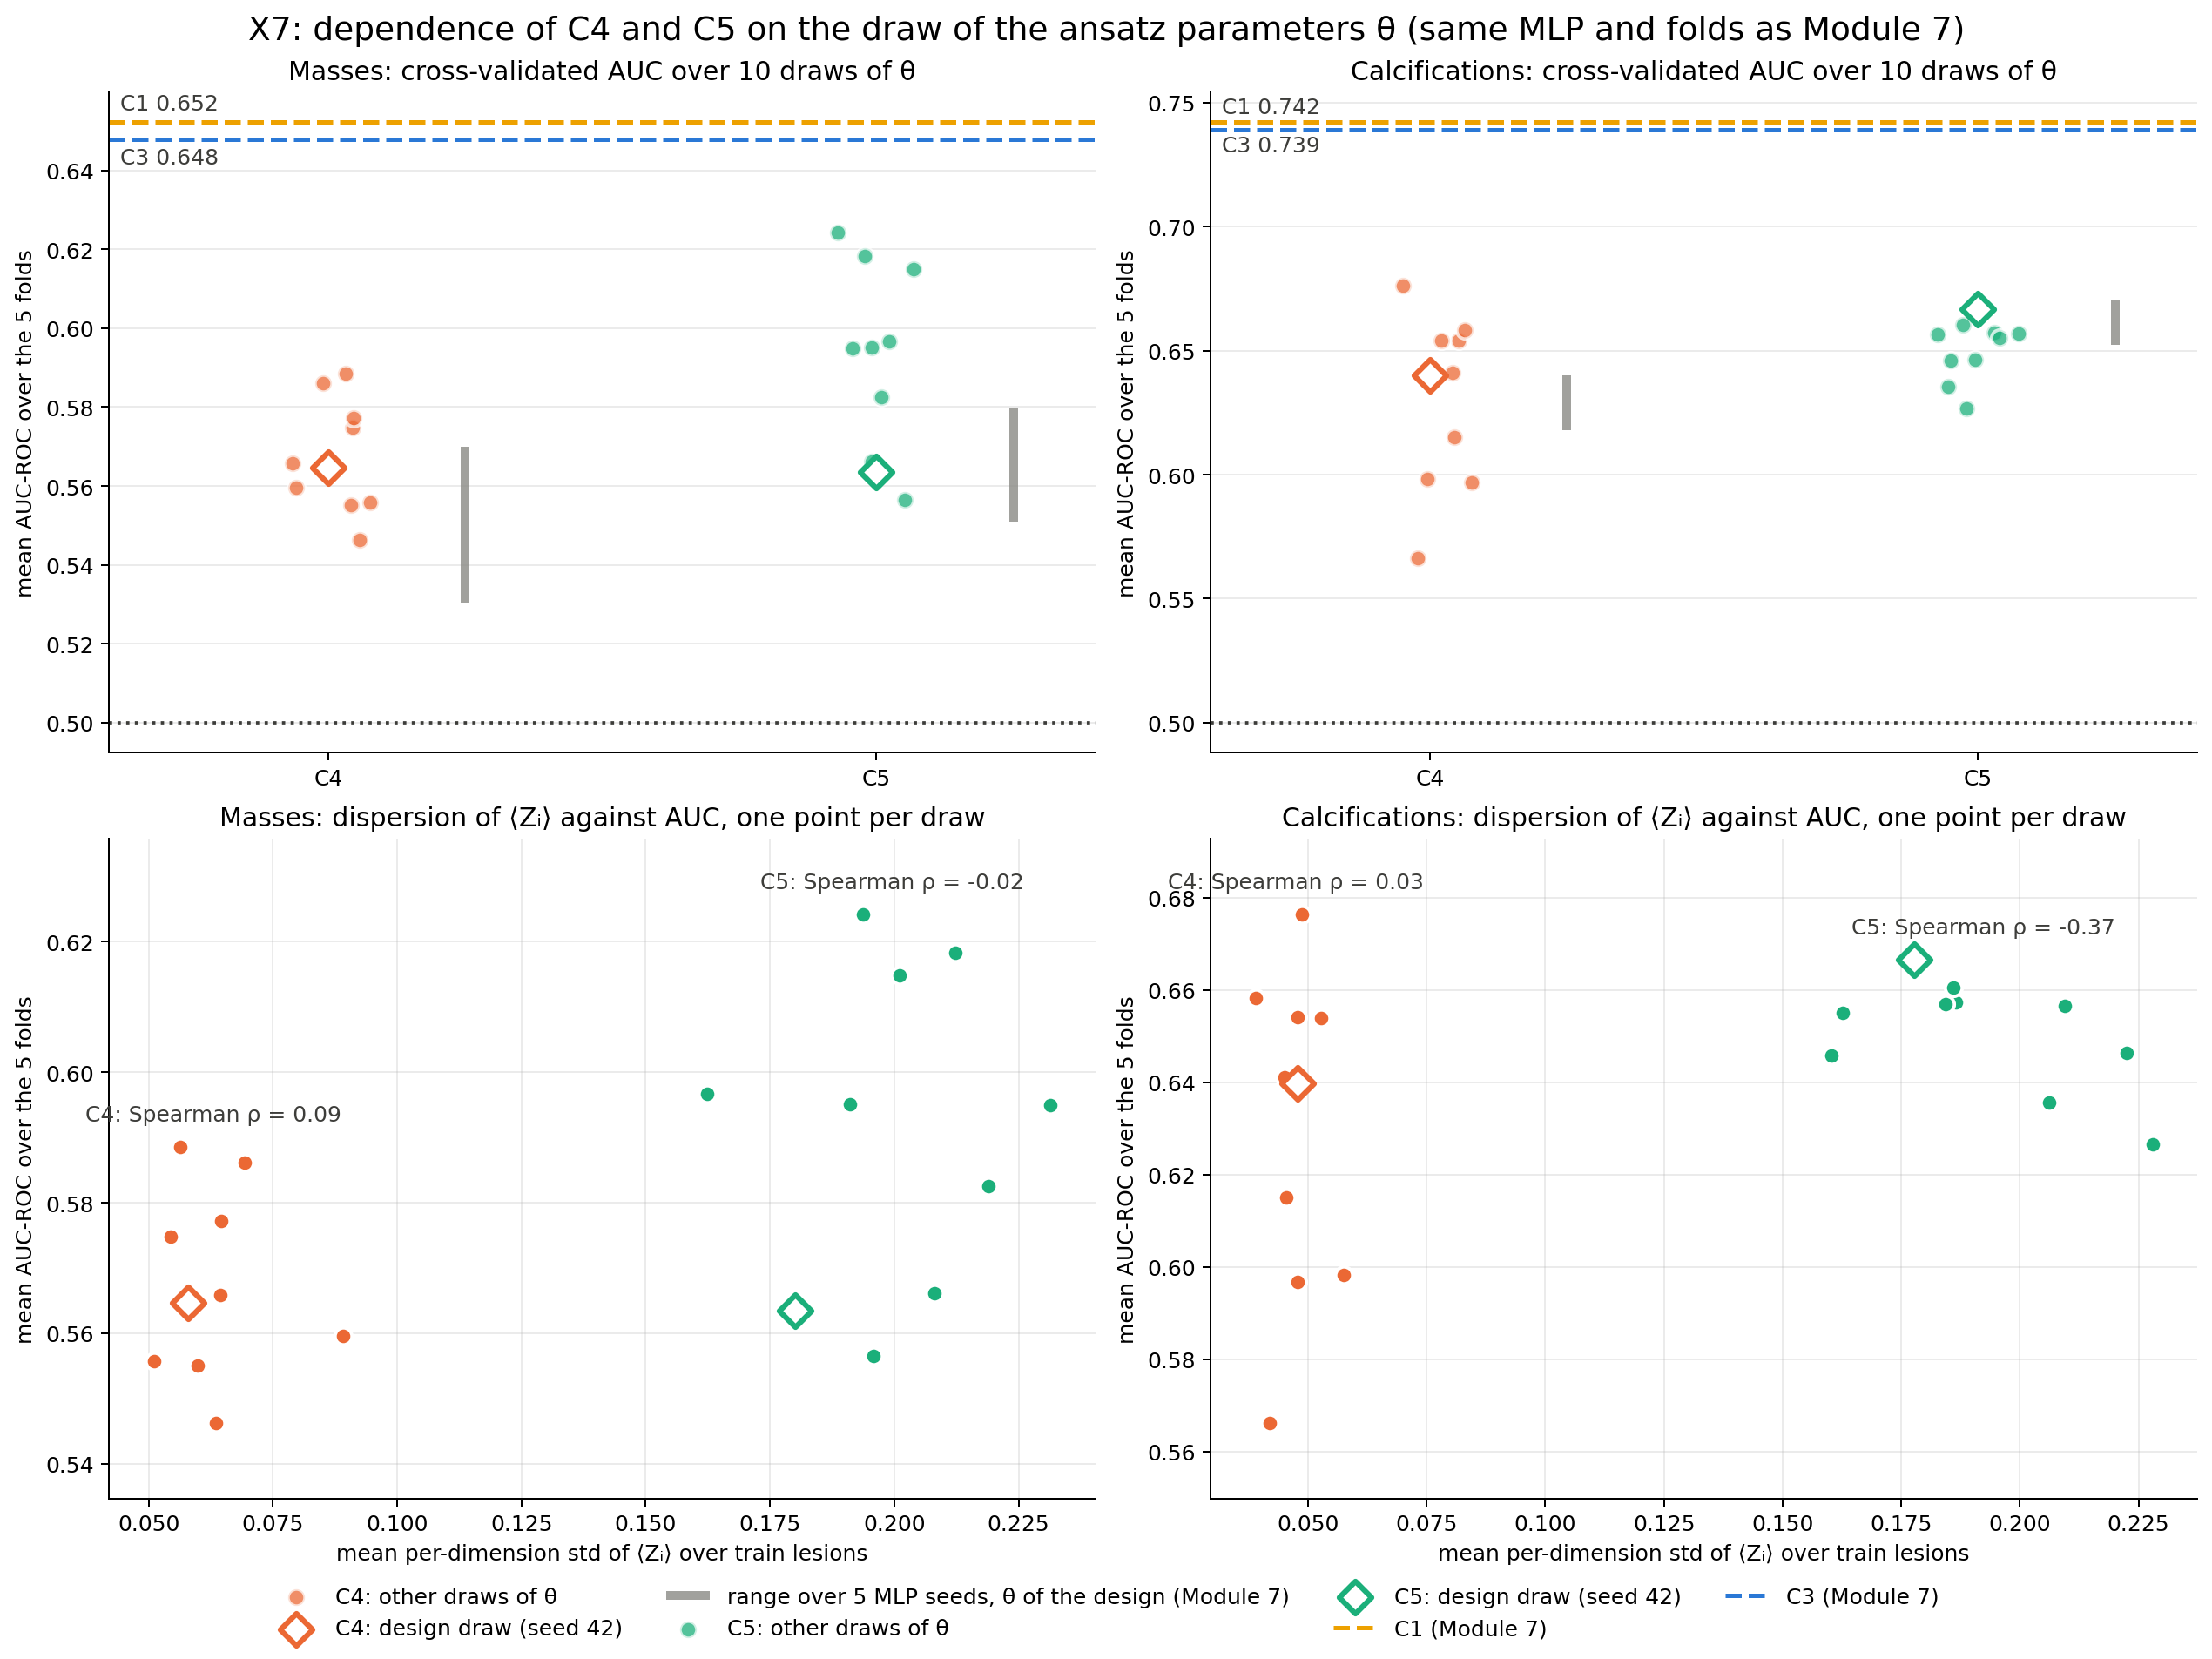
\includegraphics[width=\textwidth]{Figures/X7_theta_draws.png}
\caption{Distribución del AUC en validación cruzada a lo largo de diez sorteos aleatorios independientes de $\boldsymbol\theta$ para C4 y C5 en masas y calcificaciones.}
\label{fig:x7_theta_draws}
\end{figure}

% fuente: H-054; X8_test.csv, X8_test_diferencias.csv, X8_theta_entrenado.csv
% Generado por Code/tools/tablas_latex.py desde X8_test.csv, X8_test_diferencias.csv, X8_cv_por_fold.csv y 7_cv_resumen.csv. No editar a mano: volver a correr el script.
\begin{table}[H]
\centering
\small
\caption{Efecto de entrenar $\theta$ junto con el MLP: de $\theta$ fijo (M7) a $\theta$ entrenado.}
\label{tab:x8_theta}
\begin{adjustbox}{max width=\linewidth}
\begin{tabular}{l c c c c}
\toprule
Mapa & AUC en VC & AUC en prueba & IC 95\,\% (entrenado) & Entrenado $-$ C1 en prueba \\
\midrule
\multicolumn{5}{l}{\textit{Masas}} \\
\quad C4 & 0.565 $\to$ \textbf{0.568} & 0.530 $\to$ \textbf{0.533} & [0.468, 0.598] & \textbf{\boldmath $-$0.118 [$-$0.194, $-$0.043]} \\
\quad C5 & 0.563 $\to$ \textbf{0.612} & 0.581 $\to$ \textbf{0.585} & [0.518, 0.656] & \textbf{\boldmath $-$0.066 [$-$0.116, $-$0.019]} \\
\multicolumn{5}{l}{\textit{Calcificaciones}} \\
\quad C4 & 0.640 $\to$ \textbf{0.694} & 0.633 $\to$ \textbf{0.674} & [0.593, 0.750] & \textbf{\boldmath $-$0.094 [$-$0.154, $-$0.033]} \\
\quad C5 & 0.667 $\to$ \textbf{0.687} & 0.652 $\to$ \textbf{0.671} & [0.588, 0.745] & \textbf{\boldmath $-$0.098 [$-$0.147, $-$0.048]} \\
\bottomrule
\end{tabular}
\end{adjustbox}
\par\smallskip
\parbox{0.95\linewidth}{\footnotesize Mismo protocolo que el M7; solo cambia que $\theta$ se entrena desde el sorteo del diseño, con gradientes exactos del simulador. En negritas, el mayor AUC de cada par y las diferencias frente a C1 cuyo intervalo no contiene el cero.}
\end{table}


% fuente: H-054; X8_test.csv, X8_test_diferencias.csv, X8_costo_gradiente.csv
El entrenamiento conjunto de los parámetros $\boldsymbol\theta$ junto con los pesos del clasificador, partiendo del sorteo inicial de diseño, produce únicamente ganancias marginales que no resultan estadísticamente significativas, según se muestra en el cuadro~\ref{tab:x8_theta}. En el conjunto de prueba, la ganancia en AUC respecto a $\boldsymbol\theta$ fijo es de $+0.003$ [$-0.06$, $0.07$] en C4 masas (0.530 a 0.533), $+0.004$ [$-0.05$, $0.06$] en C5 masas (0.581 a 0.585), $+0.041$ [$-0.03$, $0.10$] en C4 calcificaciones (0.633 a 0.674) y $+0.020$ [$-0.04$, $0.08$] en C5 calcificaciones (0.652 a 0.671), abarcando en todos los casos el cero. Las cuatro combinaciones continúan ubicándose por debajo de C1 en el conjunto de prueba, con intervalos que excluyen el cero (diferencias de $-0.118$, $-0.066$, $-0.094$ y $-0.098$). Los parámetros $\boldsymbol\theta$ experimentan desplazamientos medios reducidos (0.13 a 0.39 radianes) y la época óptima de validación se alcanza entre la 4 y la 27, indicando que los 24 parámetros adicionales aportan sobreajuste antes que capacidad discriminativa generalizable.

% fuente: H-054; X8_costo_gradiente.csv
En términos de viabilidad computacional, la obtención del gradiente exacto mediante la regla de \textit{parameter-shift} (el procedimiento exigido en procesadores cuánticos físicos, con evaluaciones en $\pm \pi/2$) demanda 48 ejecuciones de circuito por lesión (5.2\,s por muestra a $k = 12$). Esto proyecta un coste de aproximadamente 205 horas de simulación por mapa de características para 50 épocas sobre el conjunto de entrenamiento. En contraste, la diferenciación automática por retropropagación analítica sobre el vector de estado en el simulador ejecuta cada muestra en 1.4\,ms (~3\,600 veces más rápido, completando 50 épocas en ~3.4 minutos) y reproduce el Jacobiano con una discrepancia numérica de apenas $1.8 \times 10^{-15}$. No obstante, este atajo analítico solo es posible en simulación clásica mediante el acceso a las 4\,096 amplitudes complejas del estado, y no existe en un computador cuántico real debido al colapso del estado inducido por la medición (figura~\ref{fig:x8_trained_theta}).

\begin{figure}[htbp]
\centering
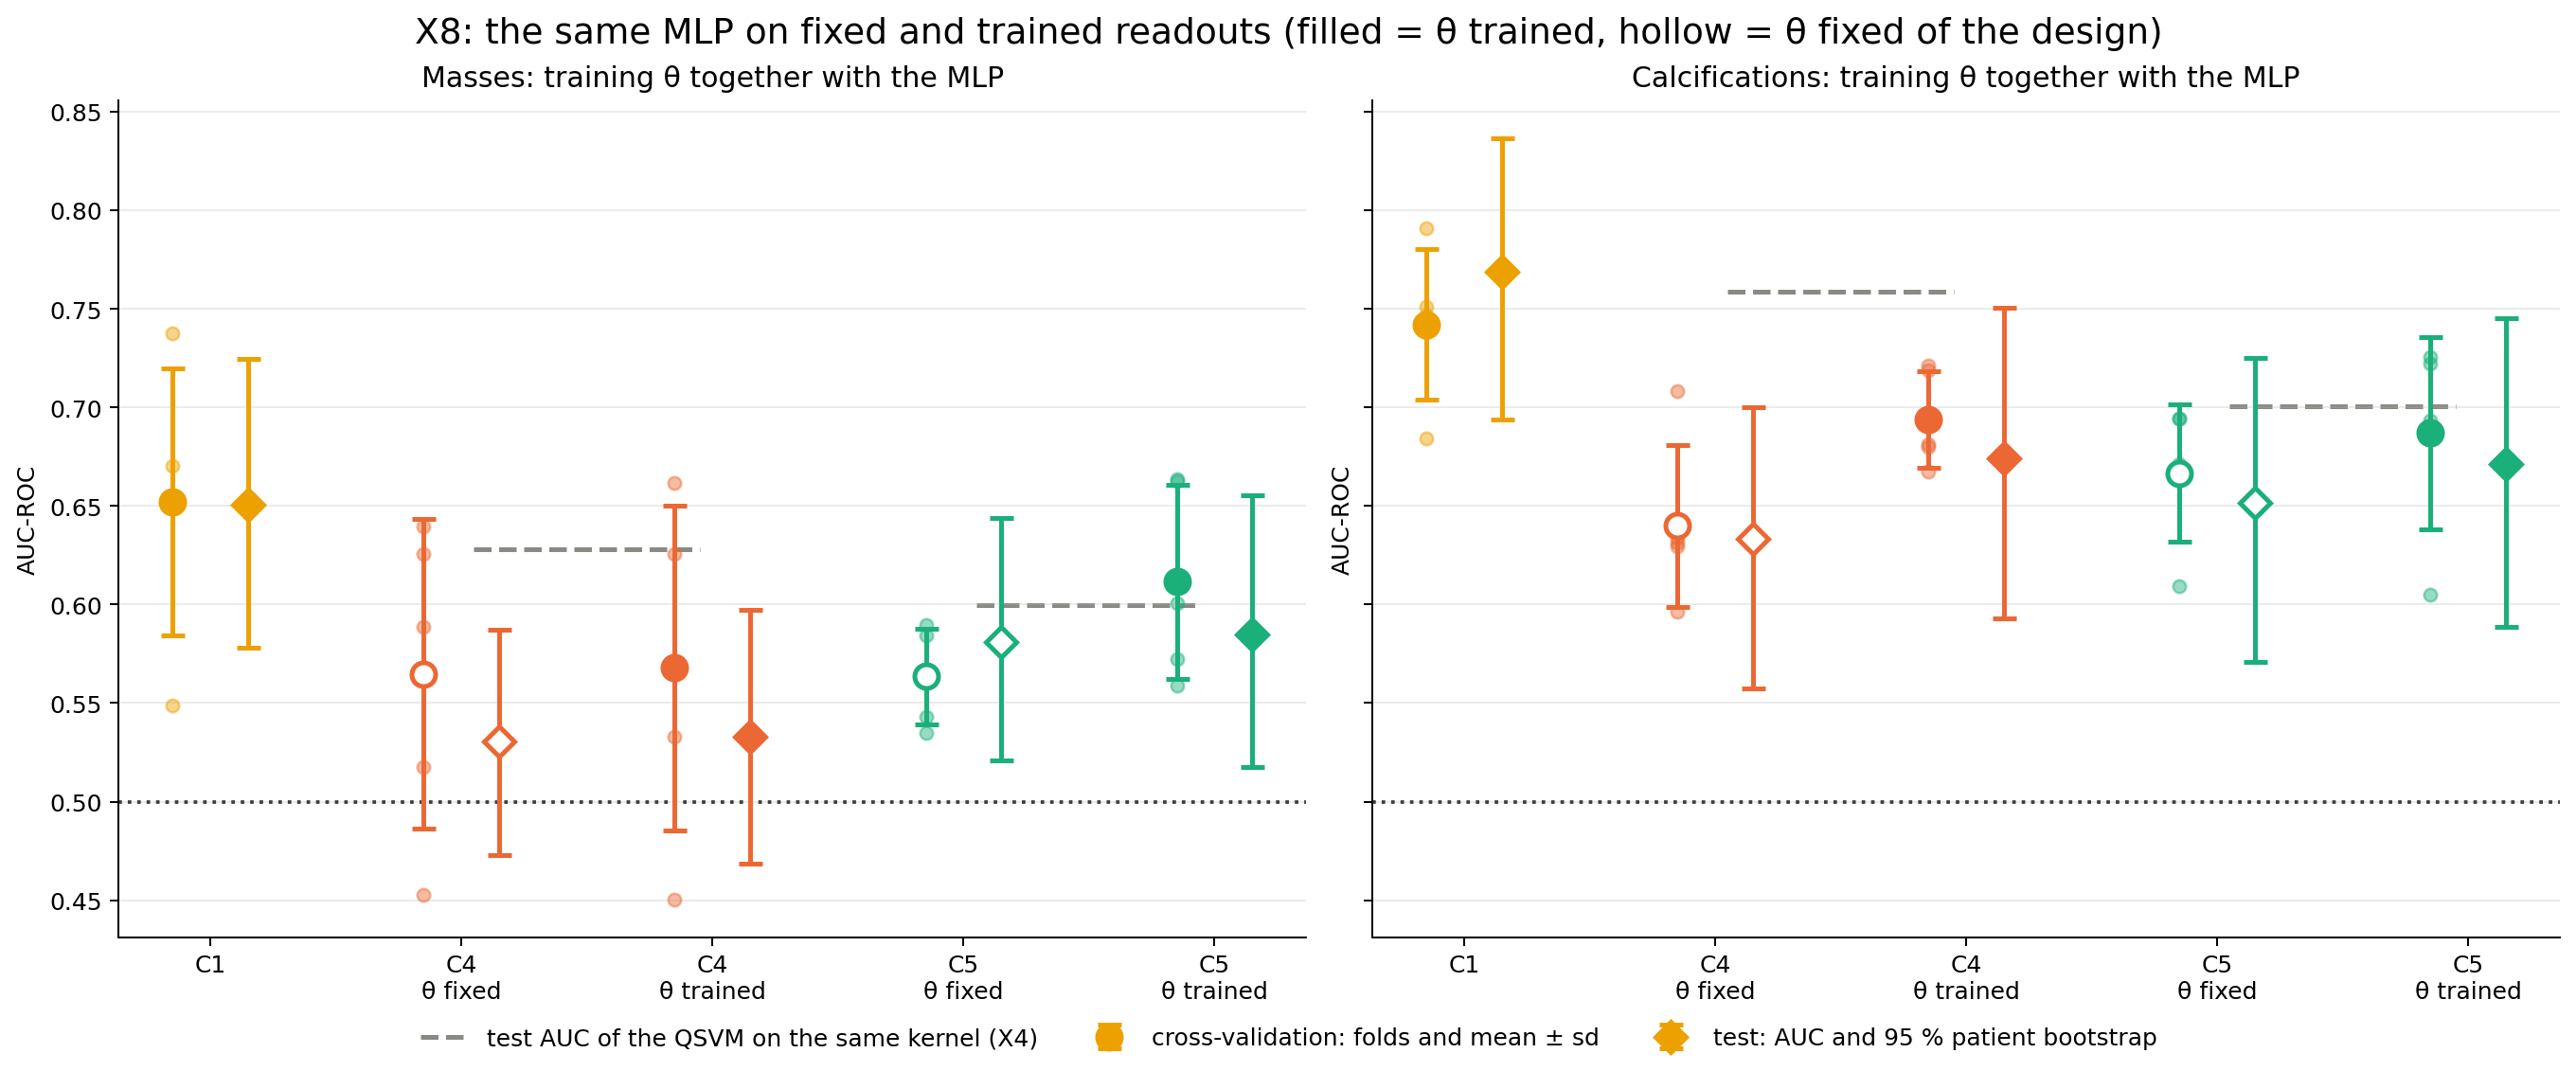
\includegraphics[width=\textwidth]{Figures/X8_trained_theta.png}
\caption{Desempeño de clasificación al entrenar los parámetros variacionales $\boldsymbol\theta$ junto con la red neuronal en comparación con $\boldsymbol\theta$ fijo, la referencia clásica C1 y el clasificador de kernel cuántico.}
\label{fig:x8_trained_theta}
\end{figure}
